\documentclass{zjureport}
% =============================================
% Part 1 Edit the info
% =============================================

\newcommand{\major}{通信工程}
\newcommand{\name}{李昊}
\newcommand{\stuid}{2014210192}
\newcommand{\newdate}{\today}
\newcommand{\loc}{北邮教二509}

\newcommand{\course}{通信系统与仿真}
\newcommand{\tutor}{赵慧}
\newcommand{\newtitle}{M序列的产生及分析}

% =============================================
% Part 1 Main document
% =============================================
\begin{document}
\thispagestyle{empty}
\begin{figure}[h]
  \begin{minipage}{0.6\linewidth}
    \centerline{
\includegraphics[width=\linewidth]{head.jpg}}
  \end{minipage}
  \hfill
  \begin{minipage}{.4\linewidth}
    \raggedleft
    \begin{tabular*}{.8\linewidth}{ll}
      专业: & \underline\major   \\
      姓名: & \underline\name    \\
      学号: & \underline\stuid   \\
      日期: & \underline\newdate \\
    \end{tabular*}
  \end{minipage}
\end{figure}

\begin{table}[!htbp]
  \centering
  \begin{tabular*}{\linewidth}{llllll}
    课程名称: & \underline\course   & 指导老师: & \underline\tutor   & 实验名称:       &  \underline\newtitle\\
  \end{tabular*}
\end{table}

% =============================================
% Part 2 Main document
% =============================================

\section{实验要求}
	利用函数testMsquence.m.      设n=9, 自己取2个不同的本原多项式(每个同学应该都不一样哦), 生成2个码字序列,画出其自相关性和互相关性。
\section{总体设计}
        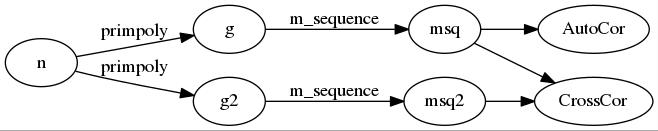
\includegraphics[width=0.8\linewidth]{graph.jpg}
\section{核心知识点}
	\begin{clause}
	\item M序列:一种产生固定周期的伪随机序列的方法
	\item 相关性: 检测信号的相似度, 可以用来验证随机性质
	\item 本原多项式: M序列发生器的结构必须是本原多项式, 可以用primpoly产生
	 \end{clause}


\section{工程结构}
    \lstinputlisting{tree.txt}

\section{结果分析}
    \begin{clause}
	\item 仿真
      \begin{center}
        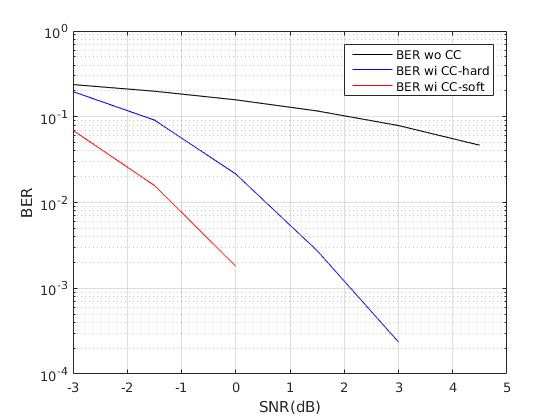
\includegraphics[width=0.8\linewidth]{main.jpg}
      \end{center}
	 \item 通过互相关可以看出俩个序列是不相关的, 符合伪随机序列
    \end{clause}
  	

\section{具体实现}
    \begin{clause}
	\item generate M sequence
	  \lstinputlisting[language=MATLAB]{code/m_sequence.m}
	 \item calculate corlerate of sequence
	  \lstinputlisting[language=MATLAB]{code/CorofCode.m}
	 \item test m sequence
	  \lstinputlisting[language=MATLAB]{code/testMsquence.m}
    \end{clause}

\end{document}
